\section{Experimental Results}
\label{sec:exp}

\begin{itemize}
	\item CPU results
		\begin{itemize}
			\item Insert-only workload
			\item Pop-only workload
			\item Mix workload
		\end{itemize}
	\item Xeon Phi results
		\begin{itemize}
			\item Insert-only workload
			\item Pop-only workload
			\item Mix workload
		\end{itemize}
	\item Explanation on why we are not fast
\end{itemize}

%we should change this subsection title
\subsection{Understanding our results}
After our results, we decided to microbenchmark cache-specific issues in order to try to improve (and fully understand) them. We first revised the memory allocation process in the XeonPhi and then we tried our data structure on a different processor microarchitecture, Intel Haswell, because of its cache-related enhancements.

\mypar{Memory allocation}
\begin{itemize}
	\item Explain memory allocation improvement
		\begin{itemize}
			\item Node size by creating nodes only for the levels needed
			\item Cache aligning. Mention that this is even more critical on the XeonPhi machine.
		\end{itemize}
	\item Graph about memory allocation improvement
\end{itemize}

% explain data + graph 
\begin{figure}
	\centering
  	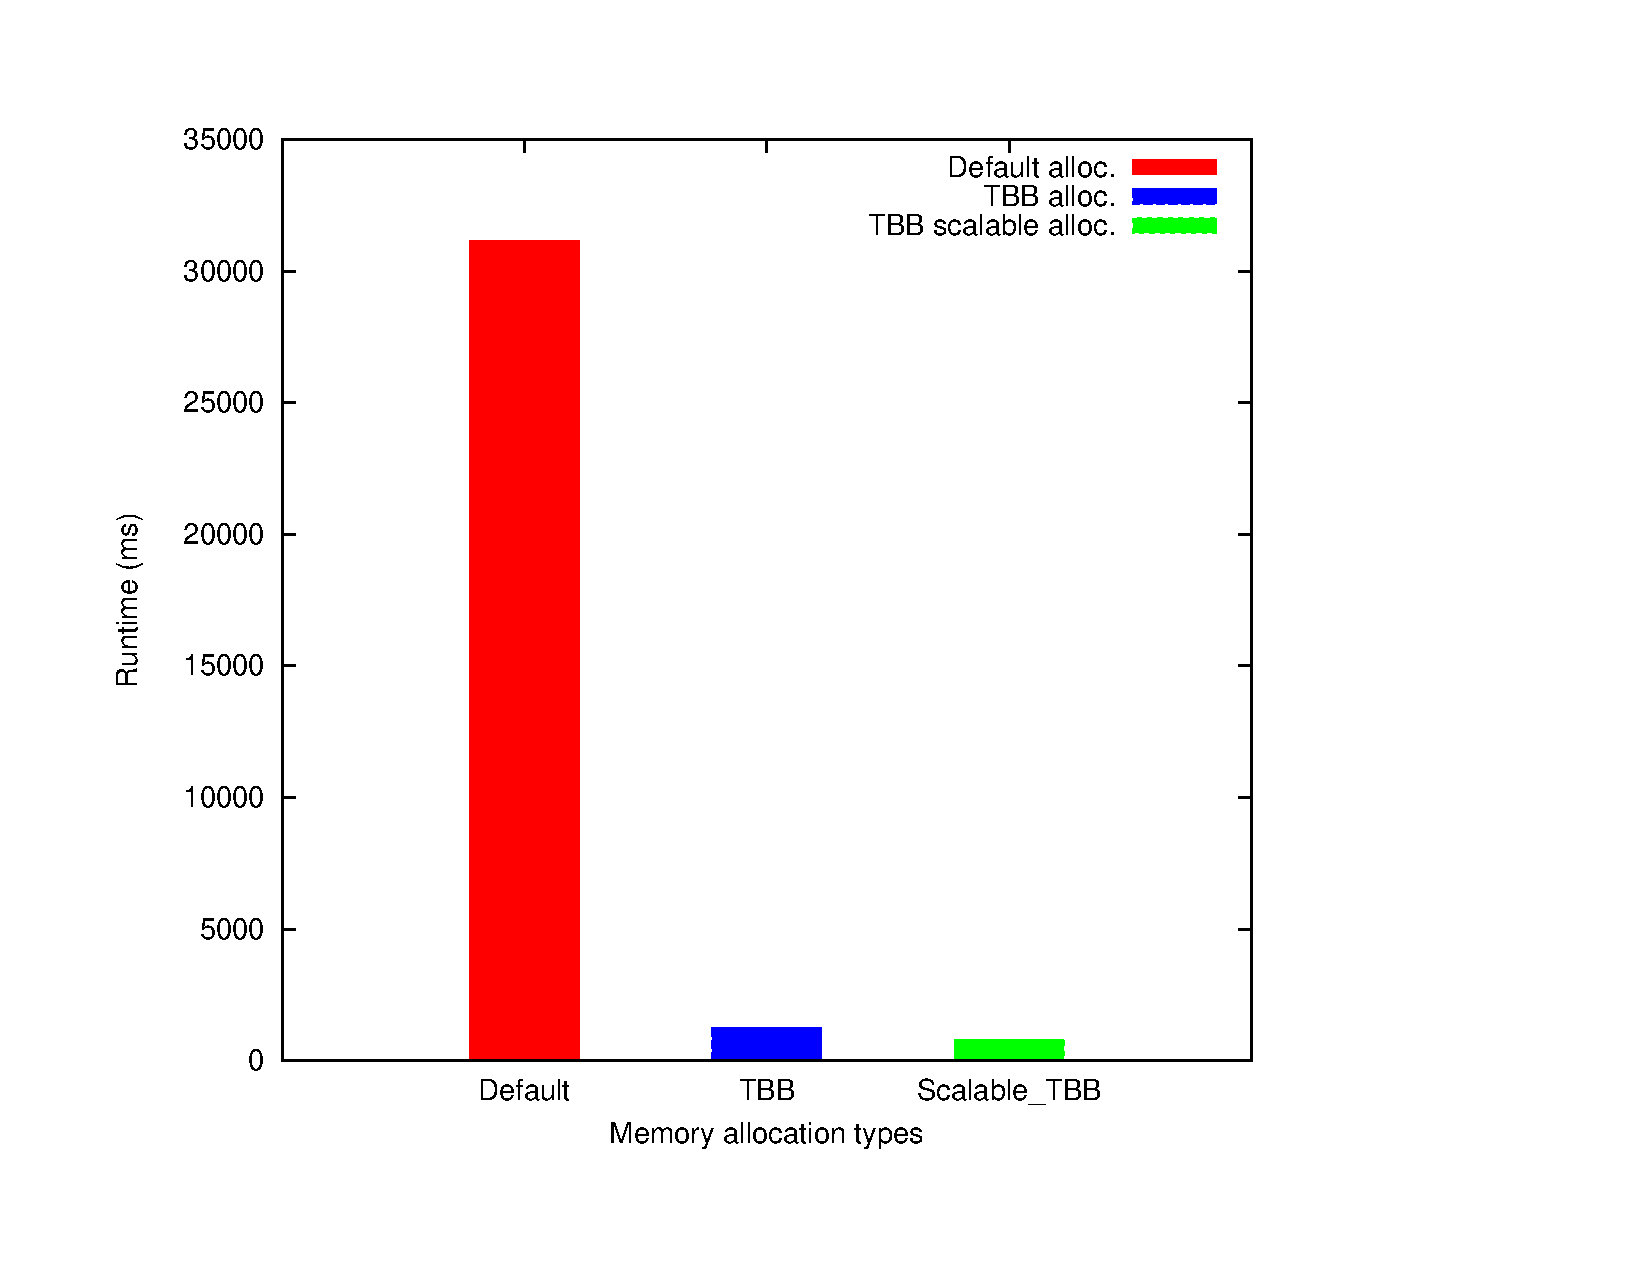
\includegraphics[scale=0.3]{../plots/mem_alloc/mem_alloc.pdf}
	\caption{Memory allocation runtime among a regular allocation, using compiler hints, and using sequential allocation with compiler hints}
	\label{fig:mem_alloc}
\end{figure}


\mypar{Operational intensity}
% recap of operational intensity
Operational intensity is defined as the ratio of the number of instructions executed to the number of memory accesses(look for citation?). If there exist many instructions per memory access, then the program is considered to have a high computational intensity i.e. compute bounded. On the other hand, if there are a small number of instructions are executed per memory access, then the program is considered to have a low computational intensity i.e. memory bounded.

% why we think it matters in our case
Our project goal was to design a simple, yet effective, priority queue. Thus, we expected to have an operational intensity dominated mainly by the number of memory accesses, and aimed to improve this. Having to move data around has a different impact on CPU architectures. We will describe and explain how our data structure behaves on Intel Haswell microarchitecture (Intel Core i7-4558U) and on Ivy Bridge microarchitecture (Intel Core i7-3820). 

% Differences between these two microarchitectures
%TODO fix bib
The Intel Haswell microarchiteture is the successor of Ivy Bridge. They have several differences but they also share many commonalities. One of the biggest change is the memory hierarchy implemented on the Intel Haswell. The cache bandwidth doubled and its memory sytem can now perform two loads and one store per cycle. The Haswell's L1 load bandwidth is of 64 bytes/cycle, its L1 store bandwidth is of 32 bytes/cycle and also L2 bandwidth to L1 has doubled (from 32 bytes/cycle to 64 bytes/cycle). Other relevant improvements are the ones related to the Translation Look-aside Buffer (TLB) which in Haswell has access to 2M shared pages. The page entry also doubled in Haswell as well as the associativity; It went from a 4-way associative TLB in Ivy Bridge to a 8-way associative TLB in Haswell. These changes are summarized on table~\ref{tab:haswell_ivy}.
%~\cite{http://ijcsit.com/docs/Volume%204/vol4Issue3/ijcsit2013040321.pdf, http://www.agner.org/optimize/microarchitecture.pdf, http://web.eecs.utk.edu/courses/fall2013/cosc530/CS530Project_intel.pdf}

\begin{table}[ht]
\footnotesize
\begin{tabular}{|l|l|l|ll}
\cline{1-3}
\multicolumn{1}{|c|}{\textbf{Metric}} & \multicolumn{1}{c|}{\textbf{Ivy Bridge}} & \multicolumn{1}{c|}{\textbf{Haswell}} &  &  \\ \cline{1-3}
L1 Load Bandwidth                     & 32 Bytes/cycle                           & 64 Bytes/cycle                        &  &  \\ \cline{1-3}
L1 Store bandwidth                    & 16 Bytes/cycle                           & 32 Bytes/cycle                        &  &  \\ \cline{1-3}
L2 Bandwidth to L1                    & 32 Bytes/cycle                           & 64 Bytes/cycle                        &  &  \\ \cline{1-3}
L2 Unified TLB                        & 4K:512, 4-way                            & 4k+2M shared: 1024, 8-way             &  &  \\ \cline{1-3}
\end{tabular}
\caption{Cache operation differences between Intel Haswell and Intel IvyBridge}
\label{tab:haswell_ivy}
\end{table}

% describe cache structure
In addition to core cache size, latency, and bandwith improvements, the Intel Haswell microarchitecture has also improved its ICache prefetch algorithms, and the way it handles conflicts. It uses hardware transactions i.e. it uses hardware to keep track of which cache lines have been read from and which have been written to. L1 cache tracks addresses read/written from/to respectively in the transactional region and it may evict address but without loss of tracking. Data conflicts occur if at least one request is doing a write, but it is detected at cache line granularity and using existing cache coherence protocol.

%~\cite{http://pages.cs.wisc.edu/~rajwar/papers/rajwar_qconsf2012.pdf}
%the Ivy Bridge has 1333MHz DRAM while the Haswell has 2133MHz DRAM
While running our priority queue benchmark on these two different architectures, we observed different behaviours. The running times when using an Intel IvyBridge processor dramatically increases due the increase of the total amount of instructions and cache misses. Everytime we need to perform an insertion, we first have to search for the adecuate place within the SkipList. The average of the SkipList nodes fit in a 64-byte cache line but the ones containing pointers in upper levels don't. On the other hand, when we used an Intel Haswell processor, running times were much less than in the IvyBridge processor. This is mainly due to the improvements done on cache operations. In this case, our data structure can take advantage of such improvements by loading more SkipList nodes into the caches that can also be used by other threads.

% explain data + graph + core architecture
\begin{figure}\centering
%  	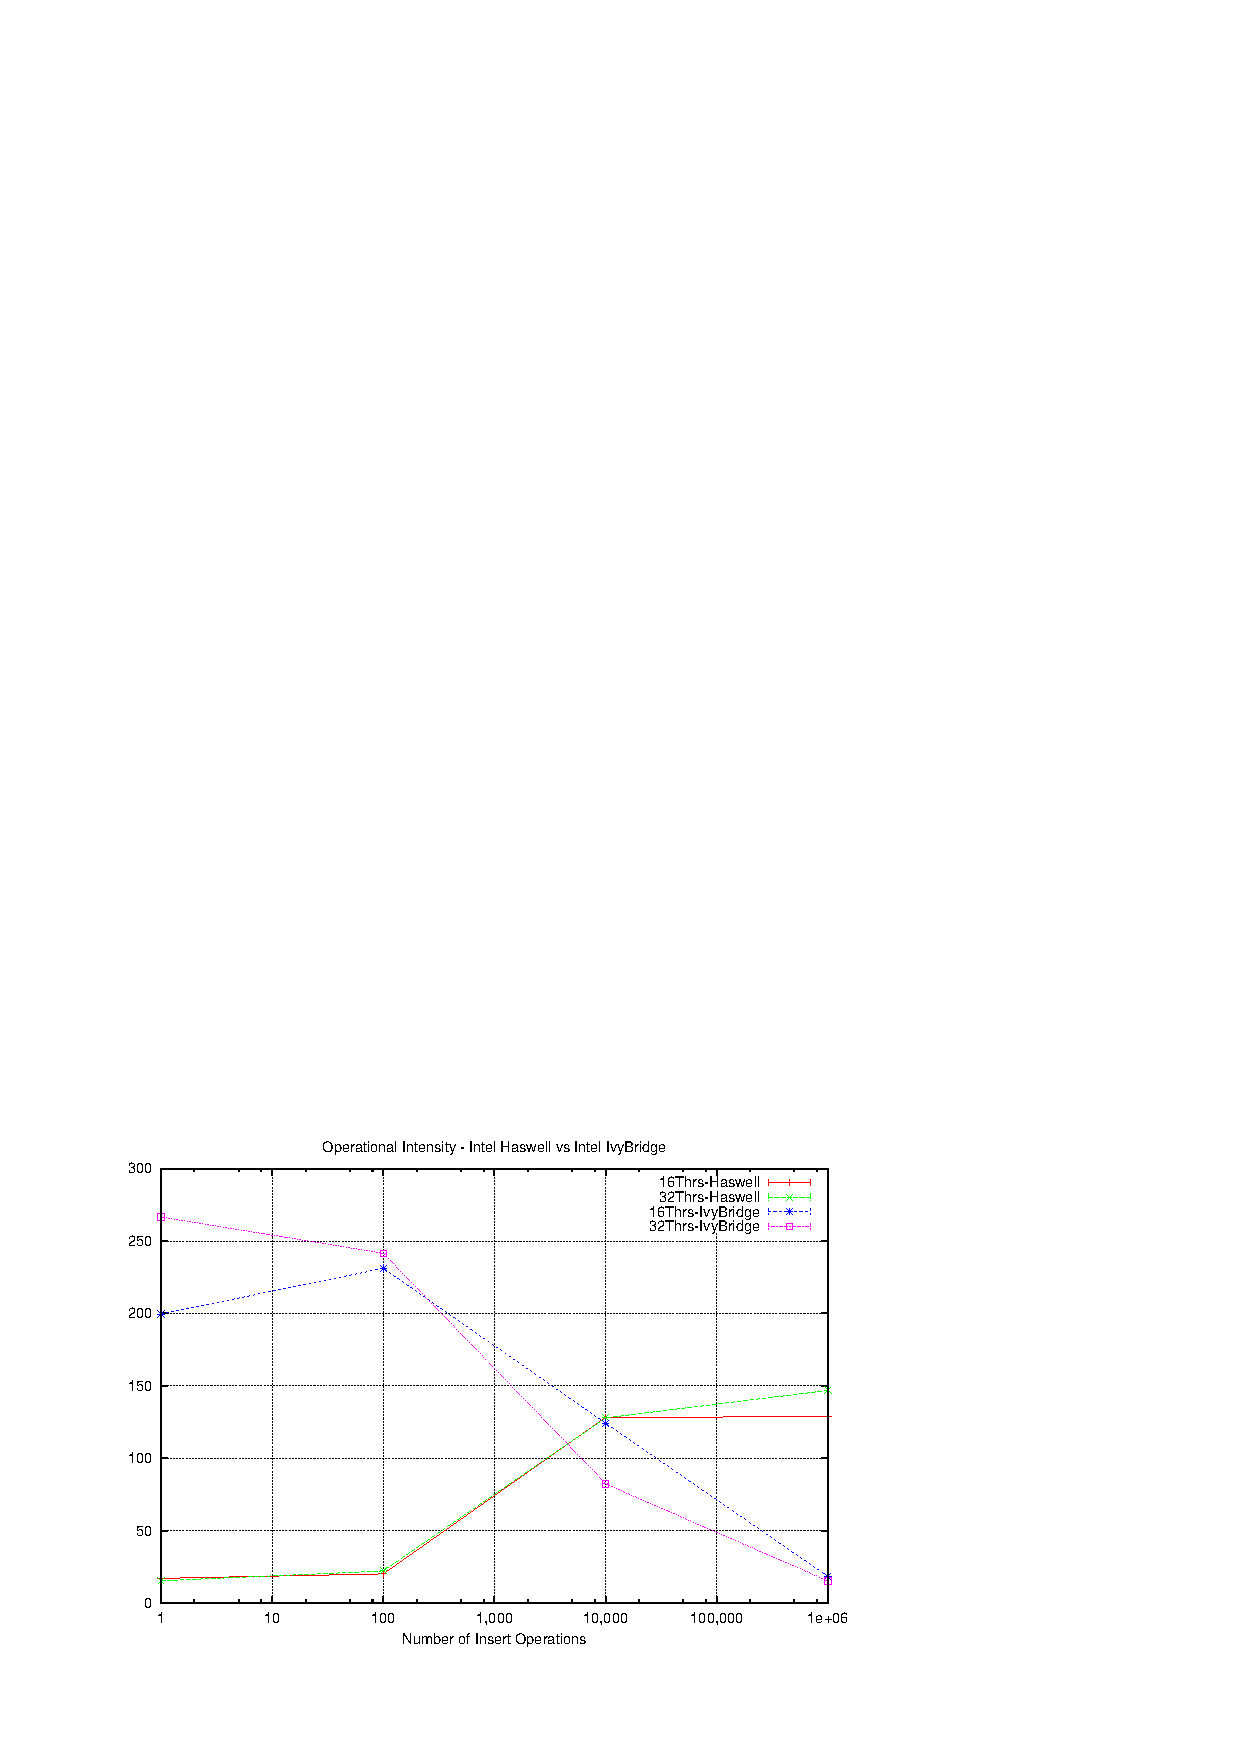
\includegraphics[scale=0.3]{../plots/haswell-ivybridge/haswell_ivybridge.pdf}
	\caption{Op. Intensity in Intel Haswell and Intel IvyBridge microarchitectures}
	\label{fig:haswell_ivybridge}
\end{figure}

Figure~\ref{fig:haswell_ivybridge} shows how operational intensity behaves when running different amounts of insert operations over such microarchitectures. It can be noted that when performing a small number of operations, our data structure is CPU bounded on an IvyBridge processor, but memory bounded on a Haswell processor. This is because in the former we have a small number of cache-misses against a really high number of instructions whether in the latter we observed a low operational intensity because we need less number of instructions for performing such tasks. When we increase the number of operations, the IvyBridge processor gets many more cache-misses compared to the Haswell one. Thus, in the former one our data structure becomes memory bounded and in the latter one CPU bounded.

\subsection{Evaluation on Xeon Phi}
\begin{figure}
	\centering
	\begin{subfigure}[b]{0.475\columnwidth}
		\centering
		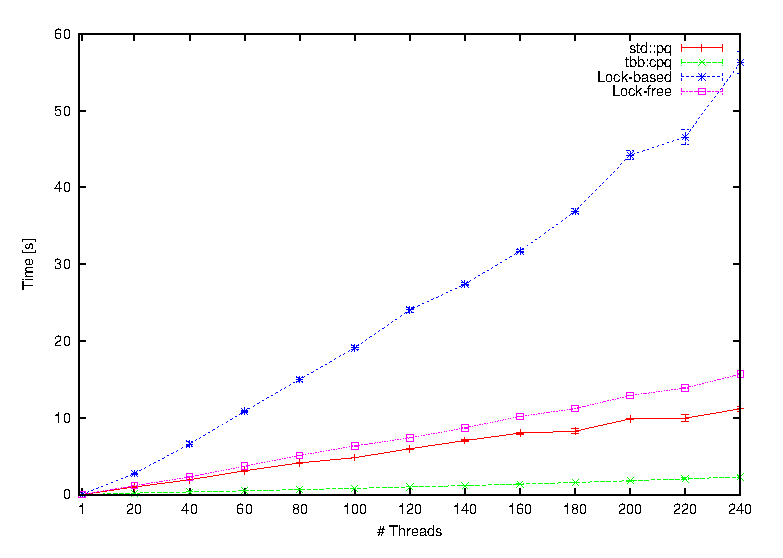
\includegraphics[width=\textwidth]{../plots/xp_push/runtime_push}
		\caption{PUSH}
		\label{fig:xp_push}
	\end{subfigure}
	\hfill
	\begin{subfigure}[b]{0.475\columnwidth}
		\centering
		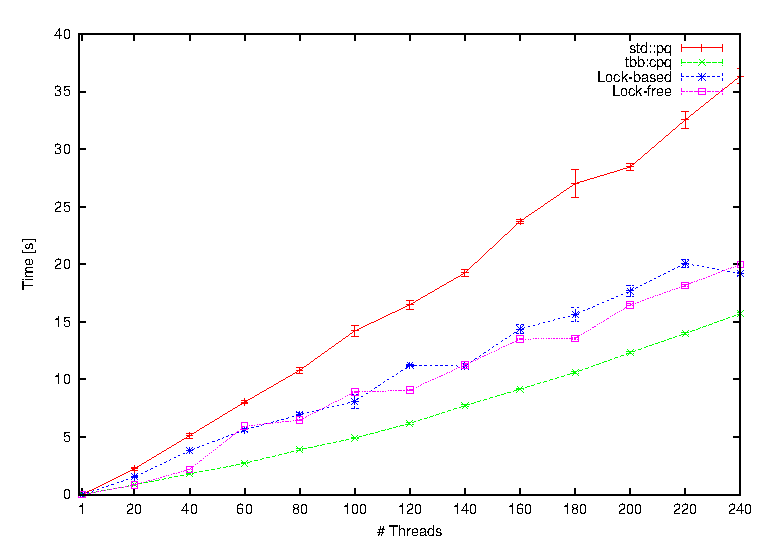
\includegraphics[width=\textwidth]{../plots/xp_pop/runtime_pop}
		\caption{POP}
		\label{fig:xp_pop}
	\end{subfigure}
	\hfill
	\begin{subfigure}[b]{0.475\columnwidth}
		\centering
		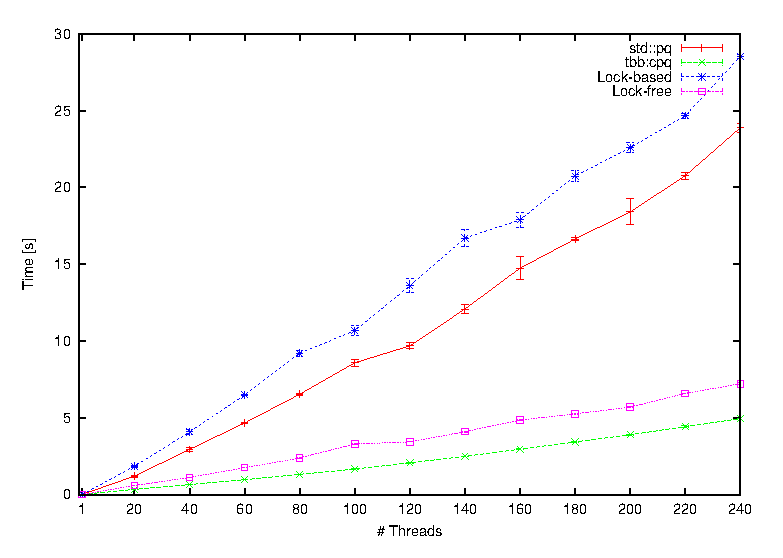
\includegraphics[width=\textwidth]{../plots/xp_mixed/runtime_mixed}
		\caption{Mixed Workload}
		\label{fig:xp_mixed}
	\end{subfigure}
	\hfill
	\begin{subfigure}[b]{0.475\columnwidth}
		\centering
		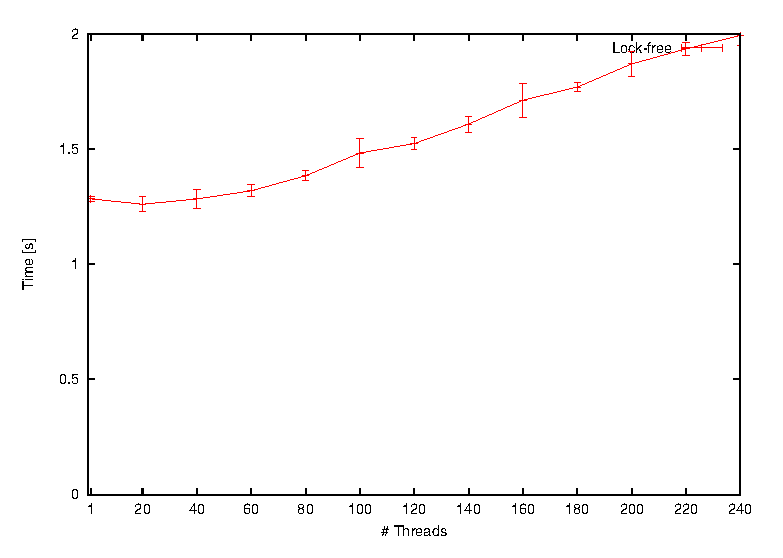
\includegraphics[width=\textwidth]{../plots/xp_contains/runtime_contains}
		\caption{Contains}
		\label{fig:xp_contains}
	\end{subfigure}
	\caption{Evaluation on Xeon Phi}
	\label{fig:three graphs}
\end{figure}
